\documentclass[12pt, oneside]{article}
\usepackage[letterpaper, margin=1in]{geometry}
\usepackage[english]{babel}
\usepackage[utf8]{inputenc}
\usepackage{amsmath}
\usepackage{amsfonts}
\usepackage{amssymb}
\usepackage{tikz}
\usepackage{tkz-fct}

\usepackage{fancyhdr}
\pagestyle{fancy}
\fancyhf{}
\rhead{\thepage \\Name: \hspace{1.5in}.\\}
\lhead{BECA / Dr. Huson / 11.2 Algebra 2 \\* 17 March 2018 \\* \textbf{Regents practice: Polynomial functions and graphs}}

\vspace{1cm}

\renewcommand{\headrulewidth}{0pt}

\title{Problem set template}
\author{Chris Huson}
\date{April 2018}

\begin{document}
%\maketitle

\subsubsection*{\\* \textnormal{Graph carefully using pencil}}

\begin{enumerate}

\item The graph of $y = f(x)$ is shown below. The function has a leading coefficient of 1.\\*
\begin{center}
    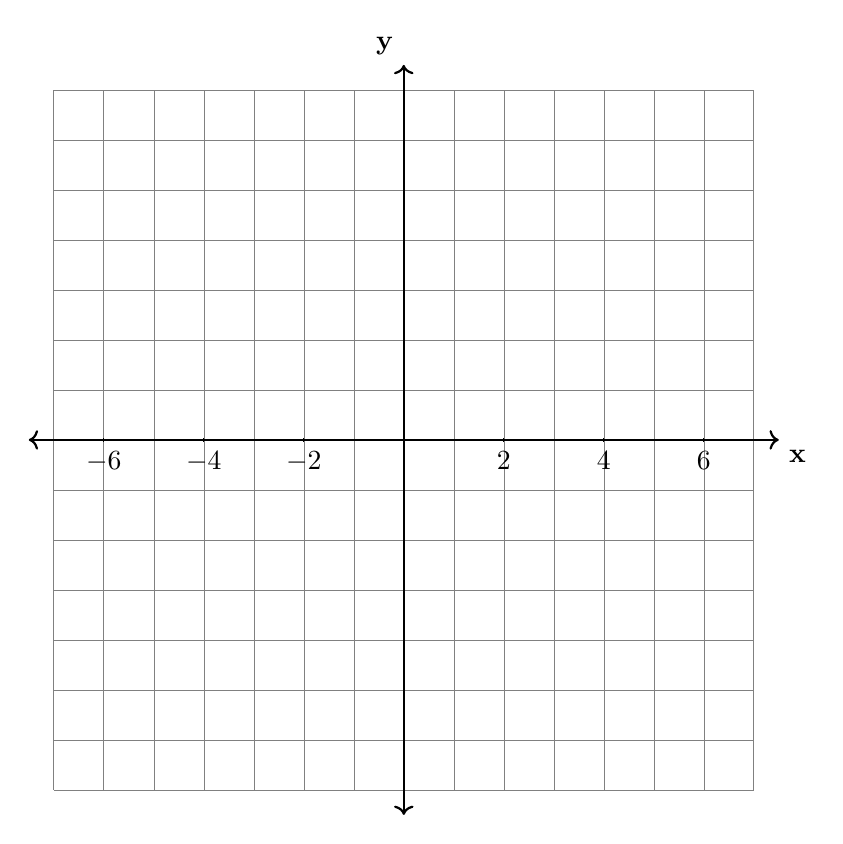
\begin{tikzpicture}[scale=2.54/4]
    \draw[step=1cm,gray,very thin] (-7,-7) grid (7,7);
    \draw[thick,<->] (-7.5,0) -- (7.5,0) node[anchor=north west] {\textbf{x}};
    \draw[thick,<->] (0,-7.5) -- (0,7.5) node[anchor=south east] {\textbf{y}};
    \foreach \x in {-6, -4, -2, 2, 4, 6} \draw (\x cm,1pt) -- (\x cm,-1pt) node[anchor=north] {$\x$};
    %\foreach \y in {5} \draw (1pt,\y cm) -- (-1pt,\y cm) node[anchor=east] {50}; %{$\y$};
    \tkzInit[xmin=-6,xmax=6,ymin=-7,ymax=7,ystep=1]   
    \tkzFct[color=black,thick,<->,domain = -4.3:5.2] {0.1*(x+3)*(x)*(x-4)};
    \end{tikzpicture}
\end{center}
Write an equation for $f(x)$.\\*[50pt]
The function $g$ is formed by translating function $f$ right 2 units. Sketch $y=g(x)$ on the same grid.\\*[10pt]
Write an equation for $g(x)$.

\newpage


\item Given that $x+1$ is a factor of $f(x)=3x^3-9x^2+8x+20$. What is the value of $f(2)$? \\*[1in]

\item What is the quotient when $2x^2-7x-40$ is divided by $x + 3$?\\*[3in]

\item Algebraically determine the values of $h$ and $k$ to correctly complete the identity stated below.
\[5x^2-x+3=(x-2)(hx+9)+k\] %\\*[3in]

\newpage
\item The zeros of a cubic polynomial function $f$ are  $-6, 0, \text{ and } 3$. The polynomial has a negative leading coefficient, $a<0$. Sketch a graph of $y = f(x)$ on the grid below.\\*
\begin{center}
    
\begin{tikzpicture}
    \draw[step=0.25in,gray,very thin] (0,0) grid (12.7,12.7);
    \end{tikzpicture}
\end{center}
Write an equation for $f(x)$.

\newpage



\item Given: $f(x)=3x^2+ 2x - 2$ and $g(x)=x-5$\\*[5pt]
Express $3x \times g(x) + 2 \times  f(x)$ as a polynomial in standard form. \\*[3in]


\item Simplify the expression $\displaystyle \frac{6x^3+9x-3}{2x-1}$, where $x \neq \frac{1}{2}$. 

\newpage
\subsubsection*{Homework}

\item Given the function $f(x)=x^3-5x^2+4x$. 
\begin{enumerate}
    \item Find the zeros of $f$.\\*[10pt]
    \item Write down $f(x)$ in factored form.\\*[50pt]
    \item Graph the function on the grid below, carefully passing through the correct $x-$ and $y$-intercepts. 
\end{enumerate}
\begin{center}
    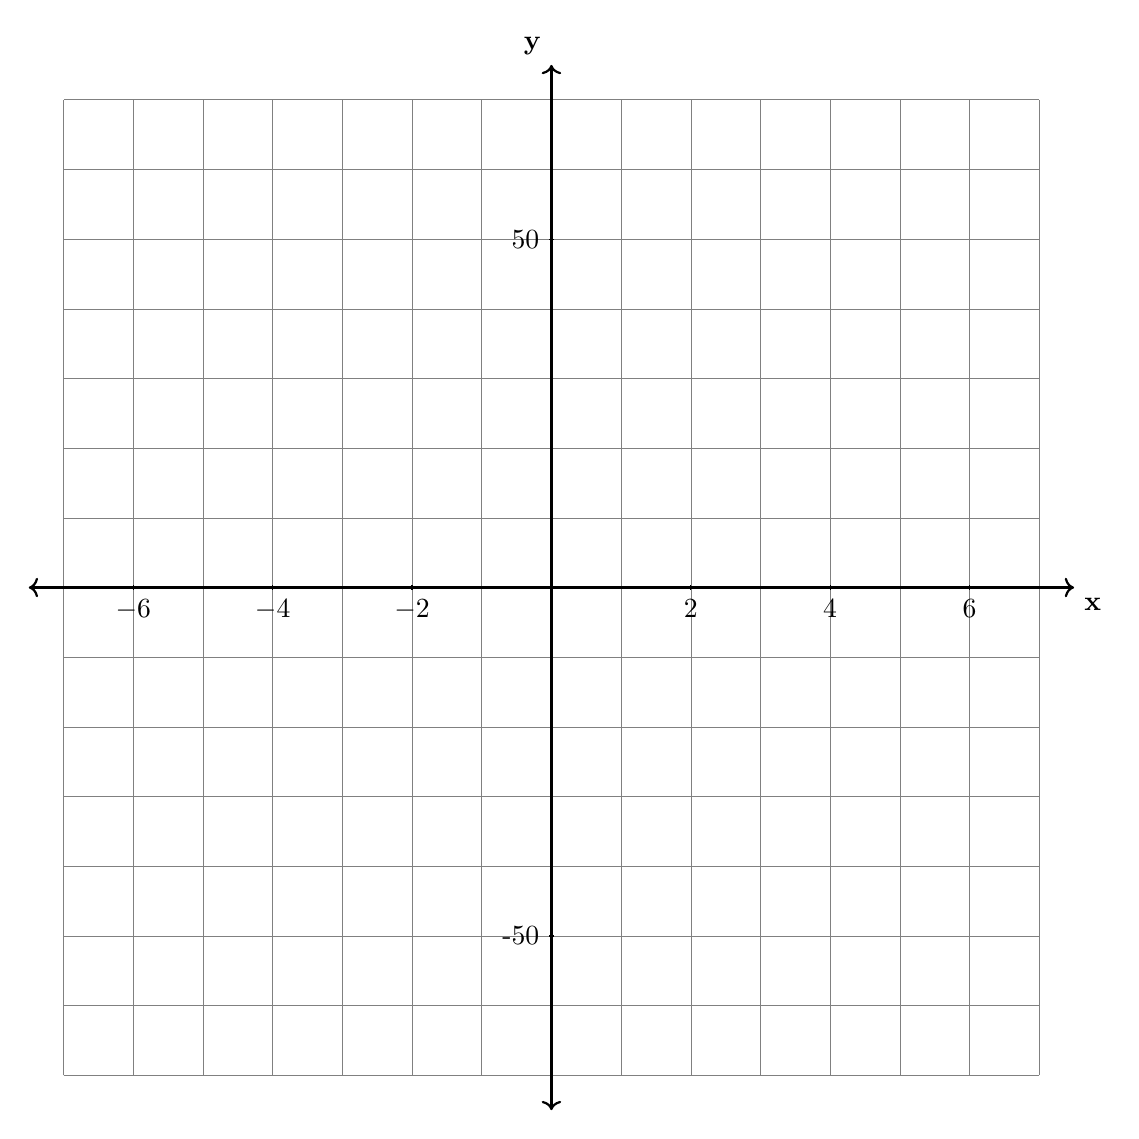
\begin{tikzpicture}[scale=3.54/4]
    \draw[step=1cm,gray,very thin] (-7,-7) grid (7,7);
    \draw[thick,<->] (-7.5,0) -- (7.5,0) node[anchor=north west] {\textbf{x}};
    \draw[thick,<->] (0,-7.5) -- (0,7.5) node[anchor=south east] {\textbf{y}};
    \foreach \x in {-6, -4, -2, 2, 4, 6} \draw (\x cm,1pt) -- (\x cm,-1pt) node[anchor=north] {$\x$};
    \foreach \y in {5} \draw (1pt,\y cm) -- (-1pt,\y cm) node[anchor=east] {50};
    \foreach \y in {-5} \draw (1pt,\y cm) -- (-1pt,\y cm) node[anchor=east] {-50};    \tkzInit[xmin=-5,xmax=5,ymin=-7,ymax=7,ystep=1]   
%    \tkzFct[color=black,thick,<->,domain = -3.4:7] {0.1*(x*x-4)*(x-5)};
    \end{tikzpicture}
\end{center}


\end{enumerate}
\end{document}